\paragraph{Gestione iscrizioni}

\label{Gestione iscrizioni ai questionari}

\begin{figure}[ht]
	\centering
	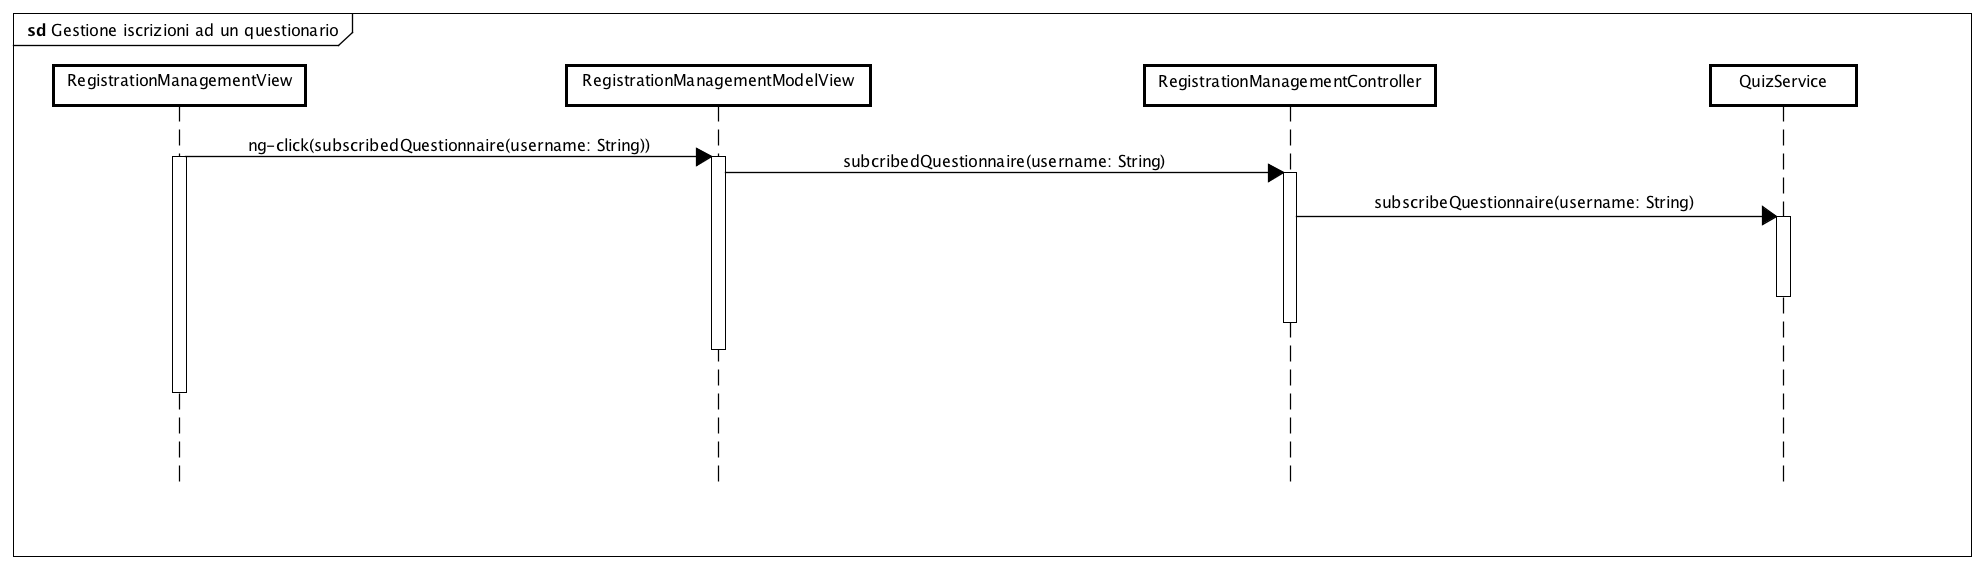
\includegraphics[scale=0.25,keepaspectratio]{UML/DiagrammiDiSequenza/Front-end/SubscriptionManagement.png}
	\caption{Gestione iscrizione al questionario di un singolo utente}
\end{figure} \FloatBarrier

Dopo che l'utente avrà selezionato un utente dalla lista di quelli iscritti al questionario, avrà la possibilità di approvare l'iscrizione. Quando l'utente preme il link di conferma iscrizione viene invocato il metodo del controller che, a sua volta, richiederà al service l'approvazione dell'iscrizione. Questa proceduta può essere ripetuta per ogni utente iscritto al questionario.